%
% Curriculum Vitæ/Résumé
% Nicolas Dubois <nicolas.c.dubois@gmail.com>
% https://nicolasdubois.com • @wo0dyn
%
% KOMA-Script: scrartcl
%
% This work is licensed under the Creative Commons Attribution-NonCommercial 4.0
% International License.
% To view a copy of this license, visit http://creativecommons.org/licenses/by-nc/4.0/.
%

\documentclass[a4paper, 11pt]{scrartcl}

\usepackage[american]{babel}
\usepackage[utf8]{inputenc}
\usepackage[pdftex]{xcolor}

\usepackage{aeguill}
\usepackage{fontawesome}
\usepackage{graphicx}
\usepackage{url}
\usepackage{vmargin}
\usepackage{xifthen}

% Bibliography

\usepackage[
  backend=bibtex,
  sorting=ydnt,   % Sort by year (descending), name, title
  style=numeric,  % numeric
]{biblatex}

\AtEveryBibitem{\clearname{author}}
\AtEveryCitekey{%
  \ifentrytype{book}{\clearname{author}}{}%
  \ifentrytype{thesis}{\clearname{author}}{}%
}
\DeclareFieldFormat{abstract}{\\\begin{quote}\begin{center}\textbf{Abstract}\end{center}#1\end{quote}}
\DeclareFieldFormat{keywords}{\begin{quote}\textbf{Keywords:}~#1\end{quote}}
\renewbibmacro*{finentry}{%
  \printfield{abstract}%
  \printfield{keywords}%
  \finentry%
}
\bibliography{publications-en.bib}
\renewcommand*{\bibfont}{\normalfont\normalsize\sffamily}

\usepackage[pdftex, colorlinks,
  pdfpagelayout=SinglePage,
  pdftitle={Curriculum Vitæ},
  pdfauthor={Nicolas C. Dubois, @wo0dyn},
  pagebackref=false,
  pdfnewwindow=true,
  bookmarksnumbered=true,
  pdfstartview={FitH},
  urlcolor=black,
  linkcolor=black,
]{hyperref}

\urlstyle{sf}
\pagestyle{empty}
\setmarginsrb
  {15mm} % left margin
  {10mm} % top margin
  {15mm} % right margin
  {10mm} % bottom margin
  {00mm} % head height
  {00mm} % head sep
  {00mm} % foot height
  {00mm} % foot skip

% Refine sections:
\let\customsection\section
  \renewcommand{\section}[1]{
  \addcontentsline{toc}{section}{#1}
  \customsection*{#1 \hrulefill}
}

% Redefine subsections:
\let\customsubsection\subsection
  \renewcommand{\subsection}[1]{
  \addcontentsline{toc}{subsection}{#1}
  \customsubsection*{\faCaretRight~#1}
}

% Redefine items:
\let\customitem\item
\renewcommand{\item}[1]{
  \customitem {\begingroup\titlefont #1\endgroup}
  \vspace{-0.3\baselineskip}
}

\definecolor{job-color}{gray}{0.4}

% Custom commands:
\newcommand{\experience}[9][building]{
  % 1: Icon
  % 2: Title
  % 3: Company
  % 4: Location
  % 5: Started on
  % 6: Finished on
  % 7: Duration
  % 8: Skills
  % 9: Description

  \ifthenelse{\equal{#1}{university}}%
      {\def\experienceIcon{\faUniversity}}%
      {\def\experienceIcon{\faBuilding}}%

  \subsubsection*{#2}
  \begin{tabular}{@{}c@{\hspace{0.5em}}l@{}}
    \experienceIcon & #3\\
    \textcolor{job-color}{\faMapMarker} & \textcolor{job-color}{#4}\\
    \textcolor{job-color}{\faCalendar}  & \textcolor{job-color}{%
      \ifthenelse{\isempty{#7}}%
        {#5 – #6}%
        {#5 – #6 · #7}%
    }
  \end{tabular}\par
  \vspace*{0.5em}
  \ifthenelse{\isempty{#9}}%
    {\vspace{0.2em}}%
    {\noindent#9\par\vspace{0.5em}}%
  \ifthenelse{\isempty{#8}}%
    {}%
    {\noindent{\footnotesize\textbf{Skills: #8}}}%
}

\newcommand{\oldxp}[8]{
  % 1: Title
  % 2: Company
  % 3: Location
  % 4: Started on
  % 5: Finished on
  % 6: Duration
  % 7: Skills
  % 8: Description
  \par\noindent{\textbf{#1}\textcolor{job-color}{~at~#2, from~#4~to~#5 (#6), in~#3.}}
}


\begin{document}

\sffamily

\begin{center}
  {\titlefont\Huge Nicolas C. Dubois (wo0dyn)}\\\vspace*{2mm}
  {\titlefont\large Senior Software Engineer, Full-remote since 2014, Guitarist}
\end{center}

\section{Overview}

\begin{minipage}[c]{32mm}
  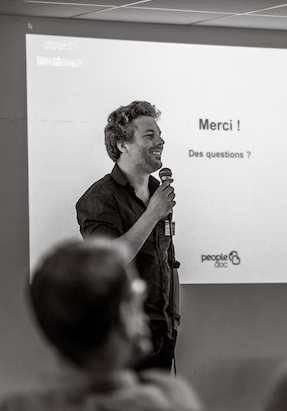
\includegraphics[width=30mm]{images/wo0dyn-at-djangocong-2018.jpg}
\end{minipage}\hfill
\begin{minipage}[c]{20cm}
  \begin{tabular}{p{48mm}@{ }p{85mm}}
    {\bfseries Address}\dotfill&
      194 Route de Labrunette\\&
      46110 Bétaille en Quercy\\&
      France\\
    {\bfseries Phone}\dotfill&
      \href{tel:+33615316404}{+336 15 31 64 04}\\
    {\bfseries Email}\dotfill&
      \href{mailto:nicolas.c.dubois@gmail.com}{nicolas.c.dubois@gmail.com}\\
    {\bfseries Personal website}\dotfill&
      \href{https://nicolasdubois.com}{https://nicolasdubois.com}\\
    {\bfseries Birth date}\dotfill&
      15 June 1979 in Nancy (France)\\
    {\bfseries Interests}\dotfill&
      Music (guitars), Basketball\\
  \end{tabular}
\end{minipage}

\section{Experience}

\experience{Lead Developer}
    {Deepki}
    {Paris, France · Full-remote}
    {Apr 2025}{Present}{}
    {Python (flask), MongoDB, Redis, AWS}{
    Lead Developer of Deepki's Impact Team:
    \begin{list}{•}{}
      \item{Tech Leadership} Participation to transversal design;
      \item{Mentoring} Regular 1:1 with 5 developers in the team (front/back).
    \end{list}
}
\experience{Senior Software Engineer}
    {Alma}
    {Paris, France · Full-remote}
    {Jun 2021}{Mar 2025}{3 yrs 10 mos}
    {Python (FastAPI/flask), PostgreSQL, Redis, GCP}{
    Feature on Alma's Buy Now–Pay Later SaaS platform (API/Dashboard):
    \begin{list}{•}{}
      \item{Onboarding} Hypermedia APIs for the merchant onboarding app;
      \item{Intl.} Internationalization/localization of Alma apps;
      \item{API} Custom API for Apple.
    \end{list}
}
\experience{Senior UI Developer, DesignOps Engineer}
    {PeopleDoc/Ultimate Software/Ultimate Kronos Group (UKG)%\footnote{\sffamily  is the result of the merger
    %of Ultimate Software (which acquired PeopleDoc in 2018) and Kronos Incorporated.}
    }
    {Paris, France \& Weston (FL)/Lowell (MA), USA · Full-remote}
    {Mar 2016}{Jun 2021}{5 yrs 4 mos}
    {Python (Django/Jinja), PostgreSQL, Redis}{
    Lots of different missions on PeopleDoc SaaS platform:
    \begin{list}{•}{}
      \item{UX/UI} Django projects referent;
      \item{Jinja} Migration to PeopleDoc's Design Language System (DLS) in templates;
      \item{Dashboard} Dashboard to monitor the adoption of DLS components;
      \item{POCs} Prototyping of several apps which turned into projects.
    \end{list}
}
\experience{Senior Software Engineer}
    {Oscaro}
    {Paris area, France · Full-remote}
    {Apr 2014}{Feb 2016}{1 yr 11 mos}
    {Python (Django/Jinja/Oscar), PostgreSQL, React.js, Redis, Elasticsearch}{
    Building a new international eCommerce platform for Oscaro.
}
\experience{Tech Lead}
    {AMG Development (GPdis Group)}
    {Toulouse area, France}
    {Oct 2009}{Apr 2014}{4 yrs 7 mos}
    {Python (Django), PostgreSQL, PHP (symfony/Magento/Zend Framework)}{
    Several internal web-apps for managing prices and clients, as well as
    maintaining the 7-shop Magento eCommerce platform (incl. Discounteo, Villatech and Pulsat).
}

\subsection{Old Experiences}

\oldxp{Tech Lead}
  {Ekinos}
  {Toulouse area, France}
  {Apr 2009}{Oct 2009}{7 mos}
  {PHP (Magento), MySQL}{Project Manager and Tech Lead on a Magento website for SAS Godard.}
\oldxp{Full Stack Developer}
  {WaterProof}
  {Toulouse area, France}
  {Nov 2007}{Apr 2009}{1 yr 6 mos}
  {PHP (Symfony), MySQL/PostgreSQL}{Foo}
\oldxp{Full Stack Developer}
  {MaisMoinsCher.com}
  {Toulouse area, France}
  {Nov 2005}{Oct 2007}{2 yrs}
  {PHP (OsCommerce), MySQL}{Foo}
\oldxp{Junior Developer}
  {Laboratoire Leibniz (IMAG)}
  {Grenoble area, France}
  {Feb 2005}{Jul 2005}{7 mos}
  {Java, MySQL}{Foo}

\subsection{Conferences}

\nocite{*}
\defbibnote{note}{\emph{
  I've attended a lot of conferences over the years and have also
  given a few talks on the Python language and its ecosystem:}}
\printbibliography[heading=none,prenote=note,type=inproceedings]

\subsection{Teaching}

\experience[university]{Web Developer/Designer}
  {Vidéoscop de Nancy}
  {Nancy, France}
  {Mar 2003}{Jun 2003}{4 mos}{}{
  Digitalization of the Human-Computer Interaction (HCI) course by Pr.~Kamel
  Smaïli (University of Lorraine) for the e-miage project.
}
\experience[university]{Tutor}
  {University Nancy 2}
  {Nancy, France}
  {Feb 2002}{Jun 2002}{5 mos}{}{
  Tutor in computer science at the Faculty of Economics and Social Sciences:
  introduction to office tools.
}

\section{Education}

\begin{description}
  \item{2004–2005: Master’s Degree in Research (DEA) “Information,
    Cognition and Learning”%, specialization in Cognitive Sciences
    }
    \par\faFileTextO{}~\fullcite{masterthesis2005}
  \item{2003–2004: Master’s Degree in Cognitive Sciences}
    \par\faFileTextO{}~\fullcite{ter2004}
  \item{2002–2003: Bachelor’s Degree in Cognitive Sciences} 
    obtained at University Nancy~2
\end{description}

\subsection{Publication}

\faBook{}~\fullcite{book2013}

\section{Skills}

\begin{tabular}{@{}c@{\hspace{0.8em}}ll@{}}
  \faDesktop  & \textbf{Environments}    & \textbf{macOS}, \textbf{GNU/Linux} (Debian/Ubuntu) \\[2pt]
  \faCode     & \textbf{Languages}       & \textbf{Python}, Unix Shells (bash/zsh), {\LaTeX} \\[2pt]
  \faGlobe    & \textbf{Web Development} & \textbf{HTML5}, \textbf{CSS3}, JavaScript/TypeScript (Vue.js), htmx \\[2pt]
  \faDatabase & \textbf{Databases}       & \textbf{PostgreSQL}, MongoDB, SQLite \\[2pt]
  \faCogs     & \textbf{Frameworks}      & \textbf{FastAPI}, \textbf{Django}, Flask \\[2pt]
  \faWrench   & \textbf{Basics}          & Elasticsearch, Java, Redis, React.js, PHP, MySQL, XML/XSL
\end{tabular}

\subsection{Languages}

\textbf{French: }Native •
\textbf{English: }Full professional proficiency •
\textbf{Spanish: }Elementary proficiency

\end{document}
